\documentclass[12pt]{article}
\usepackage[utf8]{inputenc}
\usepackage[T2A]{fontenc}
\usepackage[russian]{babel}
\usepackage{amsmath}
\usepackage{amssymb}
\usepackage{dsfont}
\usepackage[dvipsnames]{xcolor}
\usepackage{setspace}
\usepackage{multirow}
\usepackage[a4paper, outer=1.5cm, inner=1.5cm, top=1cm, bottom=1cm]{geometry}
\usepackage{graphicx}
\usepackage{skull}
\usepackage{wasysym}
\usepackage{float}
\graphicspath{{.images/}}
\usepackage{hyperref}
\hypersetup{colorlinks=true, linkcolor=blue, filecolor=magenta, urlcolor=cyan}
\usepackage[firstpage]{draftwatermark}
\SetWatermarkText{
    $\qquad\qquad\qquad\qquad\qquad$\parbox{7cm}{\begin{center}
    
\includegraphics[width = 0.08\textwidth]{lion-logo.png}\bigskip\\~\bigskip\\~\vspace{-24mm}\\~\end{center}}
}
\SetWatermarkAngle{0}
\SetWatermarkScale{1.5}
\usepackage{etoolbox}

\newtoggle{ifsolved}
\newtoggle{needhelp}
\newcounter{num}
\setcounter{num}{1}

\newcommand{\newnum}{\par\textbf{\textnumero\arabic{num}}\stepcounter{num}}
\newcommand{\sol}{\vspace{3mm}\par\textbf{Решение: }}
\newcommand{\ans}{\vspace{3mm}\par\textbf{Ответ: }}
\newcommand{\hint}{\vspace{3mm}\par\textbf{Подсказка: }}
\newcommand{\mode}[1]{
\ifstrequal{#1}{0}{\togglefalse{ifsolved}\togglefalse{needhelp}}{\ifstrequal{#1}{1}{\togglefalse{ifsolved}\toggletrue{needhelp}}{\ifstrequal{#1}{2}{\toggletrue{ifsolved}\togglefalse{needhelp}}{\toggletrue{ifsolved}\toggletrue{needhelp}}}}} %if 0 - if 1 - if 2 - else
%\newenvironment{problem}[8]{%#1, #2, #3
%\parbox{\linewidth}{\vspace{4mm}\ifstrequal{#4}{(лёгкая)}{\newnum\textbf{.}}{\newnum\textbf{*.} } \\ #5}
%\iftoggle{ifsolved}{\sol #6}{}
%\iftoggle{ifsolved}{\ans #7}{}
%\iftoggle{needhelp}{\hint #8}{}}

\newenvironment{problem}[8]{%#1, #2, #3
\parbox{\linewidth}{\vspace{5mm}\ifstrequal{#4}{(лёгкая)}{\newnum\textbf{.}}{\newnum\textbf{*.} } \\ #5}
\iftoggle{ifsolved}{\sol #6}{}

\iftoggle{ifsolved}{\parbox{\linewidth}{\ans #7}}{}
\iftoggle{needhelp}{\parbox{\linewidth}{\hint #8}}{}}

\newenvironment{mylist} %custom list
{ \begin{itemize}
    \setlength{\itemsep}{0pt}
    \setlength{\parskip}{0pt}
    \setlength{\parsep}{0pt}     }
{ \end{itemize}                  }

\newenvironment{homeass}[1]{\vspace*{-1.5cm}
\iftoggle{ifsolved}{
    \section*{\center{Решение домашнего задания к #1.}}
}{
    \section*{\center{\textcolor{Sepia}{Домашнее задание к #1}}}
} \vspace{7mm}\large}

\parindent=0pt
\pagestyle{empty}
%$\!$[\arabic{class}.\arabic{num}]
%\ifnumcomp{\value{counter}}{>}{1}{true}{false}
%\definecolor{Gray}{gray}{0.9}
%\definecolor{mypink}{RGB}{219, 48, 122}
%\newcolumntype{g}{>{\columncolor{Gray}}p{2.8cm}}

\begin{document}
\large
\mode{7}
%0 for problems without hints
%1 for problems + hints
%2 for problems + solutions + answers
%else: show all

{\centering\section*{СПИСОК ЗАДАЧ}}

{\centering\subsection*{\smallskip\\\textcolor{green}{\textbf{Полезные вещи, которые можно и нужно копипастить:}}}}

\subsection*{\textcolor{Emerald}{\textbf{Полезные шпаргалки по LaTeXу:}}}

\textbf{Пример вставки рисунка:}

\begin{minipage}{\linewidth}
    \begin{minipage}{0.54\linewidth}
    см. рисунок справа\\
    Текст к собственно пикче, примерно всегда это либо развёрнутое описание, либо большая часть решения задачи --- стремимся экономить пространство, если это можно сделать.
    \end{minipage}
    \hspace{0.05\linewidth}
    \begin{minipage}{0.4\linewidth}
    \begin{figure}[H] 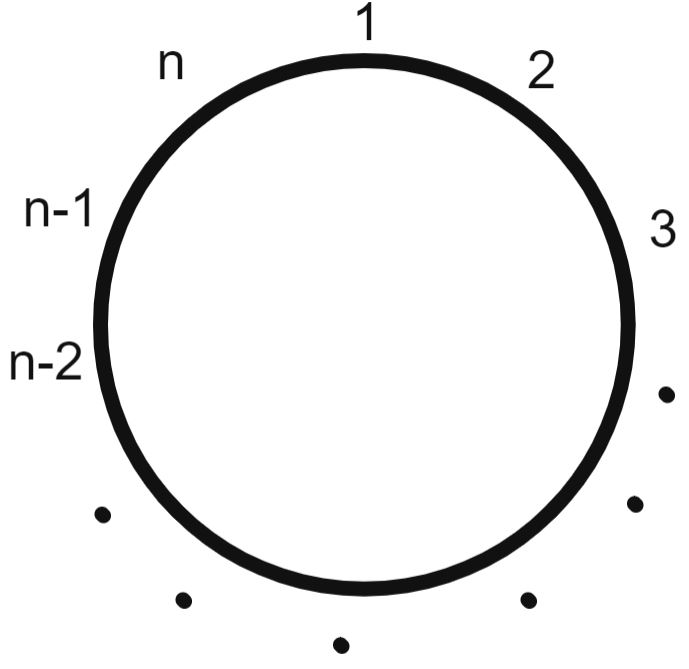
\includegraphics[width=\linewidth]{sol3} %тут поменять имя пикчи
    \end{figure}
    \end{minipage}
\end{minipage}

\textbf{Дефолтные математические знаки и символы:}\\
$\geqslant$,
$\leqslant$,
$a^{b}$,
$x_{i}$,
$\sqrt{a}$,
$\frac{a}{b}$,
$\displaystyle \frac{a}{b}$,
$\cdot$
$\;\Rightarrow\;$,
$\;\Leftrightarrow\;$,
$1{,}2$.
О промежутках:
$a\!b$,
$a\,b$,
$a\:b$,
$a\;b$,
$a\quad b$.

\textbf{Стандартные система и совокупность уравнений / неравенств:}\\
$\left\{
\begin{aligned}
f(x) &= 0 \\
g(x) &= 1
\end{aligned}\right.$

$\left[\begin{aligned}
&\left\{\begin{aligned}
f(x) &\geqslant a \\
g(x) &= b
\end{aligned}\right.\\
&\left\{\begin{aligned}
f(x) &< a \\
g(x) &= -b
\end{aligned}\right.
\end{aligned}\right.$

\subsection*{\textcolor{Emerald}{\textbf{Не математическое, но полезное:}}}
% комментарий в любом месте документа, который нигде не будет видно. Можно использовать для написания заметок-вопросов по задачам
\textbf{Пример таблицы:}

\begin{tabular}{|c|c|c|}
\hline
    $a$ & $b$ & текст
\\\hline
    $c$ & $d$ & мораль
\\\hline
\end{tabular}\\

\textbf{Отступы:} между\smallskip\\ строками\medskip\\ \textbf{Тире} --- это три дефиса.\\
\textbf{Списки:}
\begin{mylist}
\item [$\bullet$] это был пункт а
\item [2)] а это уже пункт номер 2 с изменённым заголовком
\end{mylist}

\subsection*{\textcolor{Emerald}{\textbf{Всё, неупомянутое выше (или если просто что-то не так):}}}
\begin{mylist}
\item [$\bullet$] Решение отдельных вопросов касательно ТеХа нужно искать в \href{https://www.mccme.ru/free-books/llang/newllang.pdf}{Львовском}.

\item [$\bullet$] Найти произвольный символ, который нужен, можно в \href{http://detexify.kirelabs.org/classify.html}{Detexify}.

\item [$\bullet$] Если возникли сомнения при решении, ответ практически ко всем задачам можно проверить с помощью \href{https://www.wolframalpha.com/}{WolframAlpha}.

\item [$\bullet$] Если в задаче нужно создать картинку, то лучше пока отложить эту задачу. Все графики планируется централизованно нарисовать (или перерисовать) в геогебре.

\item [\textcolor{brown}{\textbf{!!}}] Важно ставить \textcolor{red}{\textbf{$\spadesuit$}}
(или просто red) в тело задачи в случае серьёзных вопросов к решению и какой-то вопиющей лажи.

\item [\textcolor{brown}{\textbf{!!}}] Важно ставить \textcolor{olive}{\textbf{$\spadesuit$}}
(или просто olive) в тело задачи в случае не самого удачного текста и кривых отступов.
\end{mylist}

\subsection*{\textcolor{Violet}{\textbf{Комментарии:}}}% а также невидимые комментарии - так можно оставлять заметки-вопросы прямо в задаче, чтобы потом было понятно, в чём вопрос.
\begin{mylist}
\item [$\skull$] Переставлять задачи местами --- очень плохая идея.

\item [$\smiley$] При двойном клике по тексту pdf справа происходит автоматический переход к этому месту в латех-коде, а для обратного перехода можно нажать стрелку вправо (висит сверху между pdf и латех-кодом).

\item [$\smiley$] Если есть размышления, дописывать red/olive к задаче или не дописывать, то лучше всё-таки дописать.

\item [$\skull$] Самое плохое, что можно сделать --- написать в любое поле из трёх (НаписанноеРешение/ВерныйОтвет/Подсказка) только половину того, что надо, никак это не отметить, и потом пойти дальше.\\ Нужно в этот момент писать red/olive в случайном месте задачи, чтобы потом вычислить это с помощью Ctrl+F по всему документу (и это то, что потом будет делаться долго и тщательно)
\end{mylist}

\newpage
\setcounter{num}{1372}

\hypertarget{9.4}{{\centering\section*{\bigskip\\\textcolor{Blue}{\hyperlink{start2}{\textcolor{Blue}{9.4}} Числовые функции.}\vspace{-5mm}}}}

\begin{problem}{Область определения и область значений функции.}{9.4.1}{79I red многопунктовая}{(лёгкая)}
{Найти область определения для следующих функций:
\\a) $\displaystyle a(x) = \frac{x^{3} + 5x}{x^{2} + 4x + 4}$
\hfill b) $\displaystyle b(x) = \frac{2 - x}{x^{2} - 10x + 21}$
\hfill c) $\displaystyle c(x) = \frac{5x + 37}{x^{2} + 3}$
\\d) $\displaystyle d(x) = \frac{3x + 4}{x - 10}$
\hfill e) $\displaystyle e(x) = \frac{x^{3} - 4x^{2} + 5x - 7}{x^{2} - 4}$
\hfill f) $\displaystyle f(x) = \frac{1}{\sqrt{x^{2} - 5x + 6}}$
\\g) $\displaystyle g(x) = \sqrt{x^{2} - 5x + 4}$
\hfill h) $\displaystyle h(x) = \sqrt{8x - 20}$
\hfill i) $\displaystyle i(x) = \sqrt{6 + x + x^{2}}$
\\j) $\displaystyle j(x) = \sqrt{\frac{(4 - x)(x^{2} + 1)}{(x - 3)^{2}}}$
\hfill k) $\displaystyle k(x) = \frac{1}{\sqrt{x^{2} + x - 20}}$
\\ l) $l(x) = \displaystyle \sqrt{\frac{\sqrt{17 - 15x - 2x^{2}}}{x + 3}} + \frac{x + 3}{\sqrt{(x + 2)^{2}}}$
\hfill m) $y = \displaystyle \frac{x + 1}{\sqrt{-2x^{2} - 11x + 13} (9 - x^{2})}$
\\ n) $\displaystyle y = \frac{\sqrt{x + 1001}}{\sqrt{30 - x - x^{2}}}$
\hfill o) $\displaystyle y = \frac{5}{\sqrt{x^{2} + 3x - 10}} + \frac{8}{2x - 7}$
\hfill p) $y = \sqrt{30 + x - x^{2}}$}
{НаписанноеРешение}
{ВерныйОтвет}{Подсказка}
\end{problem}

\begin{problem}{Область определения и область значений функции.}{9.4.1}{9I}{(лёгкая)}
{Найти все значения $x$, для каждого из которых имеет смысл выражение $$\displaystyle \frac{4x + 2}{\sqrt{10 - x^{2} - 3x} + \sqrt{x^{2} + x - 6}}.$$

}
{НаписанноеРешение}
{ВерныйОтвет}{Подсказка}
\end{problem}

\begin{problem}{Область определения и область значений функции.}{9.4.1}{9I}{(лёгкая)}
{Найти ОДЗ для функции $u(t) = \sqrt{17t^{2} - 51t + 85}$.}
{НаписанноеРешение}
{ВерныйОтвет}{Подсказка}
\end{problem}

\begin{problem}{Область определения и область значений функции.}{9.4.1}{X}{(лёгкая)}
{Найти область значений функции $y = \sqrt{20 + x - x^{2}}$.}
{НаписанноеРешение}
{ВерныйОтвет}{Подсказка}
\end{problem}

\begin{problem}{Различные способы задать функцию.}{9.4.2}{9I}{*}
{Построить график неявной функции: $\displaystyle F(x, y) = (x - 5)(x + 1) + y(y - 2) = 0$.}
{НаписанноеРешение}
{ВерныйОтвет}{Подсказка}
\end{problem}

\begin{problem}{Различные способы задать функцию.}{9.4.2}{X}{(лёгкая)}
{Найти число точек разрыва у кусочной-заданной функции:\\ $\displaystyle \;f(x) = \left\{
\begin{aligned}
    2x^{3} - x^{2} + 2&, \text{ если } x \leqslant \frac{1}{2}\\
    \frac{1}{5}x + 1{,}9\;\;&, \text{ если } \frac{1}{2} < x < \frac{3}{2}\\
    \frac{1}{5} + \frac{3}{x}\;\;\;\;&, \text{ если } \frac{3}{2} < x \leqslant 1000\\
    0\qquad&, \text{ иначе }
\end{aligned}\right.$}
{НаписанноеРешение}
{ВерныйОтвет}{Подсказка}
\end{problem}

\begin{problem}{Свойства функций. Примеры.}{9.4.3}{9D}{(лёгкая)}
{Существует ли такая функция $f(x)$, которая строго убывает на всей своей области определения, но при этом $f(1) > f(-1)$?}
{НаписанноеРешение}
{ВерныйОтвет}{Подсказка}
\end{problem}

\begin{problem}{Свойства функций. Примеры.}{9.4.3}{9D red нельзя давать до экспонент}{(лёгкая)}
{Решить уравнение $3^{x} + 4^{x} = 7^{x}$.}
{НаписанноеРешение}
{ВерныйОтвет}{Подсказка}
\end{problem}

\begin{problem}{Свойства функций. Примеры.}{9.4.3}{9D red нельзя давать до экспонент}{(лёгкая)}
{Решить неравенство: $(x + 1) \cdot 3^{x - 2} > 45$.}
{НаписанноеРешение}
{ВерныйОтвет}{Подсказка}
\end{problem}

\begin{problem}{Свойства функций. Примеры.}{9.4.3}{9D red нельзя давать до экспонент}{(лёгкая)}
{Решить неравенство: $2^{\sqrt{5 - x}} + 3^{\sqrt{5 - x} + 1} + 4^{\sqrt{5 - x} + 2} > 20$.}
{НаписанноеРешение}
{ВерныйОтвет}{Подсказка}
\end{problem}

\begin{problem}{Свойства функций. Примеры.}{9.4.3}{9D}{(лёгкая)}
{Решить неравенство: $\,\sqrt{7 + x} \geqslant 7 - 2x$.}
{Заметим, что при $x = 2$ достигается равенство: $\sqrt{9} = 7 - 4$.\\ При этом левая часть неравенства представляет собой корень, сдвинутый вдоль оси абсцисс, а значит~--- монотонно возрастающую функцию на всей области определения ($x \geqslant -7$). Правая же часть является линейной функцией с $k = -2$, следовательно, она является монотонно убывающей функцией (на всём $\mathbb{R}$).\\
Поэтому неравенство будет выполнено правее $x = 2$ и не будет~--- левее $x = 2$. Сама же точка $x = 2$ входит в ответ, так как неравенство нестрогое.}
{$x \in [2; +\infty)$.}{Подсказка}
\end{problem}

\begin{problem}{Свойства функций. Примеры.}{9.4.3}{9D}{(лёгкая)}
{Решить уравнение: $\,\sqrt[3]{4x - 1} + \sqrt[3]{x + 1} + \sqrt[9]{x - 6} = 6$.}
{Корень произвольной степени, как чётной, так и нечётной, является монотонно возрастающей функцией от $x$. Поскольку подкоренные выражения~--- линейные двучлены с положительными коэффициентами при $x$, их рост происходит одновременно с ростом $x$, то есть функции $\sqrt[3]{4x - 1}$, $\sqrt[3]{x + 1}$, $\sqrt[9]{x - 6}$~--- монотонно возрастающие (на области их определения). По определению монотонной функции, сумма монотонно возрастающих функций монотонно возрастает. Поэтому левая часть нашего уравнения представляет собой монотонно возрастающую функцию. Вследствие этого факта, данное уравнение может или иметь единственное решение, или не иметь ни одного.\\
Однако, после пары попыток корень угадывается~--- это $x = 7$: $\;\sqrt[3]{27} + \sqrt[3]{8} + \sqrt[9]{1} = 6$.

}
{$x = 7$ является единственным решением данного уравнения.}{Подсказка}
\end{problem}

\begin{problem}{Свойства функций. Примеры.}{9.4.3}{9D red сложность явно высокая **, но задача обязательная}{*}
{Решить неравенство: $(2x^2 + 1)^5 - (3x)^5 > 3x - 2x^2 - 1$.}
{Для начала проведём двойную замену: $A(x) = 2x^2 + 1$, $B(x) = 3x$. Наше неравенство сведётся к виду $A^5 - B^5 > B - A$, или, что то же самое, $A^5 + A > B^5 + B$. Если теперь определить функцию $f(x) = x^5 + x$, то наше\\ неравенство упрощается до неравенства $f(A) > f(B)$.\\
$f(x)$~--- монотонно возрастающая на $\mathbb{R}$ функция. Действительно, $x^5$ и $x$~--- классические школьные функции, являющиеся монотонно возрастающими (на всём $\mathbb{R}$), и их сумма также монотонно возрастает. Поэтому $f(A) > f(B) \;\Longleftrightarrow\; A > B$.\\
Итак, мы доказали, что наше нер-во тождественно неравенству $2x^2 + 1 > 3x \;\Rightarrow\; 2x^2 - 3x + 1 > 0 \;\Rightarrow\; (2x - 1)(x - 1) > 0 \;\Rightarrow\; x\in(-\infty; \frac12) \cup (1; +\infty)$.}
{$x\in(-\infty; \frac12) \cup (1; +\infty)$.}{Начать решение стоит с двойной замены (ввести $A(x)$ и $B(x)$)}
\end{problem}

\begin{problem}{Свойства функций. Примеры.}{9.4.3}{9D}{*}
{Определить число корней уравнения в зависимости от $a$:\\ $\sqrt{50 - t} + \sqrt{37 - t} + \sqrt{26 - t} + \sqrt{17 - t} + \sqrt{10 - t} + \sqrt{5 - t} + \sqrt{2 - t} + \sqrt{1 - t} = a$.

}
{Рассмотрим функцию $f(t) = \sqrt{c - t}$. Независимо от величины $c$, функция $l(t) = c - t$ является строго убывающей на $\mathbb{R}$. Функция же $s(t) = \sqrt{t}$, в свою очередь, является строго возрастающей (на своей области определения $t\geqslant0$).\\ Таким образом, интересующий нас вопрос~--- какой характер поведения у функции $f(t) = s(l(t))$. Но понятно, что композиция монотонно возрастающей и монотонно убывающей функций (в любом порядке) будет монотонно убывающей функцией.\\ Поэтому все корни, участвующие в уравнении, монотонно убывают с ростом $t$, а значит, и сумма всех этих корней монотонно убывает с ростом $t$ (на их области определения).\smallskip\\
Теперь рассмотрим ОДЗ: для того, чтобы все подкоренные выражения были неотрицательны, мы должны иметь $\;t\leqslant50,\, t\leqslant 37,\, \ldots,\, t\leqslant 1$. Поэтому $t\leqslant 1$.\\ Найдем значение левой части при $t = 1$: $\sqrt{49} + \ldots + \sqrt{1} + \sqrt{0} = 1 + \ldots + 7 = 28$.\\
Следовательно, при $a = 28$ уравнение имеет один корень $t = 1$.\\ При $a > 28$ уравнение также будет иметь 1 корень, поскольку левая часть уравнения, согласно доказанному выше, имеет область определения $(-\infty; 1]$ и является монотонно убывающей функцией. При $a < 28$, так как область определения левой части уравнения лежит левее $t = 1$, уравнение не будет иметь решений.}
{При $a \geqslant 28$ уравнение имеет одно решение, иначе~--- решений нет.}{Подсказка}
\end{problem}

\begin{problem}{Свойства функций. Примеры.}{9.4.3}{9D red многопунктовая экспоненты надо поместить отдельно}{(лёгкая)}
{Указать промежутки, на которых функция монотонно возрастает/убывает:\\
a) $y = x^2 + 2x + 5$\hfill b) $\displaystyle y = 3 - \frac{6}{x - 5}$\hfill c) $y = 3^{x^2 - 4x + 11}$.}
{a) $x^2 + 2x + 5 = (x + 1)^2 + 4$.\\ $(x + 1)^2$ монотонно возрастает при росте $x$, начиная с $x = -1$, то есть на $[-1; \infty)$, и монотонно убывает до $x = -1$, то есть на $(-\infty; -1]$.\medskip\\
b) Алгебраическая дробь $\frac{6}{x - 5}$ положительна при $x > 5$ и отрицательна при $x < 5$, а при $x = 5$ не определена. При $x > 5$ c ростом $x$ знаменатель растёт, поэтому сама дробь уменьшается, поэтому $y(x)$ растёт и приближается к 3.\\ При $x < 5$ с ростом $x$ знаменатель растёт, поэтому сама дробь по модулю растёт, поэтому $y(x)$ растёт. В самой точке $x = 5$ функция не определена, поэтому возрастание происходит только на интервалах.\medskip\\
c) Мы знаем, что функция $f(x) = 3^{x}$ монотонно возрастает при росте $x$ на всей своей области определения. Поэтому выясним, в каких областях растёт функция $x^2 - 4x + 11$. $\;x^2 - 4x + 11 = (x - 2)^2 + 7$. Поэтому она монотонно убывает на промежутке $(-\infty; 2]$ и монотонно возрастает на промежутке $[2; +\infty)$.\\
Следовательно, то же самое происходит и с функцией $y(x)$.}
{$y(x)$ монотонно убывает на $(-\infty; -1]$ и монотонно возрастает на $[-1; +\infty)$.\medskip\\
$y(x)$ монотонно возрастает на интервалах $(-\infty; 5)$ и $(5; +\infty)$.\medskip\\
$y(x)$ монотонно убывает на $(-\infty; 2]$ и монотонно возрастает на $[2; +\infty)$.}{Подсказка}
\end{problem}

\begin{problem}{Чётные и нечётные функции.}{9.4.4}{X}{(лёгкая)}
{Для функции $\displaystyle y(x) = x + \frac{1}{x}\,$ найти точки разрыва и область значений.}
{НаписанноеРешение}
{ВерныйОтвет}{Подсказка}
\end{problem}

\begin{problem}{Кубический корень.}{9.4.6}{9I}{(лёгкая)}
{Решить уравнение $\,\sqrt[3]{7x^3 - 2x^2 + 3} = x + 1$.}
{Для решения иррационального уравнения воспользуемся безопасным равносильным переходом~--- возведением в нечётную степень. Поскольку степень нечётна, знаки проверять не нужно.\\ Возводим обе части уравнения в куб, получаем:
$7x^3 - 2x^2 + 3 = (x + 1)^3$.\\ Раскрываем скобки, приводим подобные члены: $7x^3 - 2x^2 + 3 = x^3 + 3x^2 + 3x + 1 \;\Rightarrow\; 6x^3 - 5x^2 - 3x + 2 = 0$. Такое можно решить с помощью теоремы Безу: достаточно отметить, что сумма коэффициентов равна 0 $\Rightarrow\; x = 1$ является корнем, поэтому $6x^3 - 5x^2 - 3x + 2 = (x - 1)(6x^2 + x - 2) = 0$. Квадратное уравнение $6x^2 + x - 2 = 0$ решаем через дискриминант: $D = 1 + 48 = 49 \Rightarrow x = \frac{-1 \pm 7}{12} \Rightarrow x = -\frac23;\; x = \frac12$.\smallskip\\
Итого мы нашли три корня уравнения: $x = -\frac23;\; x = \frac12;\; x = 1$.\\ Поскольку потеря знака у нечётной степени невозможна, все корни подходят.}
{Уравнение имеет 3 корня: $x = -\frac23;\; x = \frac12;\; x = 1$.}{Подсказка}
\end{problem}

\begin{problem}{Кубический корень.}{9.4.6}{9I}{(лёгкая)}
{Решить уравнение $\,\sqrt[4]{x^4 - 2x^3 - x^2 - 3x + 11} = x - 1$.}
{Для решения иррационального уравнения воспользуемся равносильным переходом~--- возведением в чётную (четвёртую) степень. Будем помнить, что, поскольку степень чётна, нужно в дальнейшем проверить знаки всех полученных выражений. После возведения в 4 степень имеем: $x^4 - 2x^3 - x^2 - 3x + 11 = (x - 1)^4$ $\Rightarrow\; x^4 - 2x^3 - x^2 - 3x + 11 = x^4 - 4x^3 + 6x^2 - 4x + 1 \;\Rightarrow\; 2x^3 - 7x^2 + x + 10 = 0$.\\
При должной внимательности замечаем, что $x = -1$ является корнем (равна 0 знакопеременная сумма коэффициентов). Раскладываем на множители исходный кубический многочлен: $\;2x^3 - 7x^2 + x + 10 = (x + 1)(2x^2 - 9x + 10) = 0$.\\
Квадратное уравнение $2x^2 - 9x + 10 = 0$ решаем через дискриминант:\\ $D = 81 - 80 = 1 \Rightarrow x = \frac{9 \pm 1}{4} \Rightarrow x = 2;\; x = 2{,}5$.\smallskip\\ Мы нашли три \textbf{потенциальных} корня: $x = -1;\; x = 2;\; x = 2{,}5$.\\ Делаем обязательную проверку, потому что в ходе решения было использовано неравносильное преобразование: \\
При $x = -1$ получаем, что корень четвёртой степени равен $-2$, что невозможно.\\
При $x = 2$ получаем 1 под корнем и 1 снаружи, проблем со знаками нет.\\
При $x = 2{,}5$ под корнем имеем $\frac{81}{16}$, снаружи $\frac32$. Итого $x = 2$ и $x = 2{,}5$ подходят.}
{Уравнение имеет 2 корня: $x = 2;\; x = 2{,}5$.}{Подсказка}
\end{problem}

\begin{problem}{Кубический корень.}{9.4.6}{9I}{(лёгкая)}
{Решить уравнение $\,\sqrt[4]{x^4 - 2x^3 - x^2 - 3x + 11} = 1 - x$.}
{Для решения иррационального уравнения воспользуемся равносильным переходом~--- возведением в чётную (четвёртую) степень. Будем помнить, что, поскольку степень чётна, нужно в дальнейшем проверить знаки всех полученных выражений. После возведения в 4 степень имеем: $x^4 - 2x^3 - x^2 - 3x + 11 = (1 - x)^4$ $\Rightarrow\; x^4 - 2x^3 - x^2 - 3x + 11 = 1 - 4x + 6x^2 - 4x^3 + x^4 \;\Rightarrow\; 2x^3 - 7x^2 + x + 10 = 0$.\\
При должной внимательности замечаем, что $x = -1$ является корнем (равна 0 знакопеременная сумма коэффициентов). Раскладываем на множители исходный кубический многочлен: $\;2x^3 - 7x^2 + x + 10 = (x + 1)(2x^2 - 9x + 10) = 0$.\\
Квадратное уравнение $2x^2 - 9x + 10 = 0$ решаем через дискриминант:\\ $D = 81 - 80 = 1 \Rightarrow x = \frac{9 \pm 1}{4} \Rightarrow x = 2;\; x = 2{,}5$.\smallskip\\ Мы нашли три \textbf{потенциальных} корня: $x = -1;\; x = 2;\; x = 2{,}5$.\\ Делаем обязательную проверку, потому что в ходе решения было использовано неравносильное преобразование:\\
При $x = -1$ подкоренное выражение равно 16, правая часть уравнения получается равной 2, поэтому $x = -1$ подходит.\\
При $x = 2$ и $x = 2{,}5$ в правой части уравнения получается отрицательная величина, поэтому эти два корня~--- посторонние. Итого подходит только $x = -1$.

}{Уравнение имеет 1 корень: $x = -1$.}{Подсказка}
\end{problem}

\begin{problem}{Кубический корень.}{9.4.6}{9D}{*}
{Решить уравнение $2017x^{2021} + 5x - 2021 = \sqrt[2021]{2021 - 2020x}$.}
{НаписанноеРешение}
{ВерныйОтвет}{Подсказка}
\end{problem}

\begin{problem}{Тождественные преобразования-2.}{9.4.7}{7A red или переписать с корнями или в рац степень}{(лёгкая)}
{Найти значение выражения $\;\displaystyle \frac{\left(2a^{\frac{1}{2}} - b^{\frac{1}{2}}\right) \cdot \left(2a^{\frac{1}{2}} + b^{\frac{1}{2}}\right)}{a - \frac{1}{4}b}\,$ при $a = 1{,}35$, $b = 8{,}64$.}
{НаписанноеРешение}
{ВерныйОтвет}{Подсказка}
\end{problem}

\begin{problem}{Тождественные преобразования-2.}{9.4.7}{79I}{(лёгкая)}
{Упростить выражение $\displaystyle \frac{p(a)}{p(14 - a)}$, если $p(x)$ определена как $p(x) = \displaystyle \frac{x(14 - x)}{x - 7}$.}
{НаписанноеРешение}
{ВерныйОтвет}{Подсказка}
\end{problem}

\begin{problem}{Тождественные преобразования-2.}{9.4.7}{79I}{(лёгкая)}
{Упростить выражение и найти его значение при $m = 11 + 6\sqrt{2}$: $$\displaystyle\;\left(\frac{\sqrt{m} - 2}{\sqrt{m} + 2} + \frac{8\sqrt{m}}{m - 4}\right) : \frac{\sqrt{m} + 2}{m - 2\sqrt{m}}.$$

}
{НаписанноеРешение}
{ВерныйОтвет}{Подсказка}
\end{problem}

\begin{problem}{Тождественные преобразования-2.}{9.4.7}{79I red в иррациональные выражения с рац. степенями}{(лёгкая)}
{Упростить выражение $\displaystyle \left(1 + 2x^{\frac{2}{3}} - \cfrac{x + x^{\frac{2}{3}}}{x^{\frac{1}{3}} + 1}\right) \cdot \cfrac{1 - x^{\frac{2}{3}}}{1 - x^{\frac{4}{3}}}\,$ и найти его значение при\\ $x = 1{,}23 + 4\sqrt{5}$.}
{НаписанноеРешение}
{ВерныйОтвет}{Подсказка}
\end{problem}

\begin{problem}{Тождественные преобразования-2.}{9.4.7}{79I}{(лёгкая)}
{Упростить выражение $\displaystyle \left(\frac{x^{8} + x^{4} - \sqrt{2}x^{2} + 2}{x^{4} - \sqrt{2}x^{2} + 1} + \sqrt{2}x^{2}\right)^{\frac{1}{2}}$ и найти его значение при $x = -\sqrt[4]{2}$.}
{НаписанноеРешение}
{ВерныйОтвет}{Подсказка}
\end{problem}

\begin{problem}{Тождественные преобразования-2.}{9.4.7}{79I}{(лёгкая)}
{Упростить выражение: $\;\displaystyle\left(\cfrac{4}{a + \cfrac{1}{b + 1/c}} : \cfrac{1}{a + \cfrac{1}{b}} - \cfrac{4}{b\, (abc + a + c)}\right)^{\!-1/2}$}
{НаписанноеРешение}
{ВерныйОтвет}{Подсказка}
\end{problem}

\begin{problem}{Тождественные преобразования-2.}{9.4.7}{79I}{(лёгкая)}
{Упростить выражение: $\;\displaystyle\left(\cfrac{t\sqrt{t + 2}}{\sqrt{t - 2}} - \cfrac{2\sqrt{t - 2}}{\sqrt{t + 2}} - \cfrac{4t}{\sqrt{t^{2} - 4}}\right)^{1/2} \!\!: \sqrt[4]{t^{2} - 4}$.}
{НаписанноеРешение}
{ВерныйОтвет}{Подсказка}
\end{problem}

\begin{problem}{Тождественные преобразования-2.}{9.4.7}{79I}{(лёгкая)}
{Упростить выражение: $\;\displaystyle\left(\frac{a\sqrt{a} + b\sqrt{b}}{\sqrt{a} + \sqrt{b}} - \sqrt{ab}\right)\left(\frac{\sqrt{a} + \sqrt{b}\:}{a - b}\right)^{2}$.}
{НаписанноеРешение}
{ВерныйОтвет}{Подсказка}
\end{problem}

\begin{problem}{Тождественные преобразования-2.}{9.4.7}{79I}{(лёгкая)}
{Упростить выражение: $\;\displaystyle\left(\frac{a - \sqrt{a^{2} - b^{2}}}{a + \sqrt{a^{2} - b^{2}}} - \frac{a + \sqrt{a^{2} - b^{2}}}{a - \sqrt{a^{2} - b^{2}}}\right) : \cfrac{4\sqrt{a^{4} - a^{2}b^{2}}}{(5b)^{2}}$.}
{НаписанноеРешение}
{ВерныйОтвет}{Подсказка}
\end{problem}

\begin{problem}{Тождественные преобразования-2.}{9.4.7}{79I red рац степени}{(лёгкая)}
{Упростить выражение: $\;\displaystyle \left(\frac{x^{\frac{1}{3}}}{x^{\frac{2}{3}} - x^{\frac{1}{3}} + 1} - \frac{3x^{\frac{1}{3}} - 1}{x + 1}\right) \cdot \frac{x + 1}{x^{\frac{2}{3}} - 1}$.}
{НаписанноеРешение}
{ВерныйОтвет}{Подсказка}
\end{problem}

\begin{problem}{Тождественные преобразования-2.}{9.4.7}{79I red рац степени}{(лёгкая)}
{Упростить выражение: $\;\displaystyle \left(\frac{2x + x^{\frac{1}{2}} y^{\frac{1}{2}}}{3x}\right)^{-1}\!\!\! \cdot \,\left(\frac{x^{\frac{3}{2}} - y^{\frac{3}{2}}}{x - x^{\frac{1}{2}} y^{\frac{1}{2}}} - \frac{x - y}{x^{\frac{1}{2}} + y^{\frac{1}{2}}}\right)$.}
{НаписанноеРешение}
{ВерныйОтвет}{Подсказка}
\end{problem}

\begin{problem}{Тождественные преобразования-2.}{9.4.7}{79I}{(лёгкая)}
{Упростить выражение: $\;\displaystyle \left(\frac{1}{(\sqrt{a} + \sqrt{b})^{-2}} - \left(\frac{\sqrt{a} - \sqrt{b}}{\sqrt{a^{3}} - \sqrt{b^{3}}}\right)^{\!\!-1}\right) : \sqrt{ab}$.}
{НаписанноеРешение}
{ВерныйОтвет}{Подсказка}
\end{problem}

\begin{problem}{Тождественные преобразования-2.}{9.4.7}{79I}{(лёгкая)}
{Упростить выражение: $\;\displaystyle \, \left(\frac{\left(\sqrt{a} + \sqrt{b}\right)^{2} - 4b}{a - b} - \left(\frac{\sqrt{a} + \sqrt{b}}{\sqrt{a} - \sqrt{b}}\right)^{\!\!-1} \right) : \frac{32b\sqrt{b}}{\sqrt{a} + \sqrt{b}}$.}
{НаписанноеРешение}
{ВерныйОтвет}{Подсказка}
\end{problem}

\begin{problem}{Тождественные преобразования-2.}{9.4.7}{79I red рац степени}{(лёгкая)}
{Упростить выражение: $\;\displaystyle \, \left(\frac{1 - c^{-2}}{c^{\frac{1}{2}} - c^{-\frac{1}{2}}} - \frac{2c^{\frac{1}{2}}}{c^{2}} + \frac{c^{-2} - c}{c^{\frac{1}{2}} - c^{-\frac{1}{2}}}\right) \cdot \left(1 + \frac{2}{c^{2}}\right)^{\!\!-2}$.}
{НаписанноеРешение}
{ВерныйОтвет}{Подсказка}
\end{problem}

\begin{problem}{Тождественные преобразования-2.}{9.4.7}{79I}{(лёгкая)}
{Упростить выражение: $\;\displaystyle \:\cfrac{\sqrt{\cfrac{1}{a + 2\sqrt{a - 2} - 1}} + \sqrt{\cfrac{1}{a - 2\sqrt{a - 2} - 1}}}{\sqrt{\cfrac{1}{a + 2\sqrt{a - 2} - 1}} - \sqrt{\cfrac{1}{a - 2\sqrt{a - 2} - 1}}}$.}
{НаписанноеРешение}
{ВерныйОтвет}{Подсказка}
\end{problem}

\begin{problem}{Тождественные преобразования-2.}{9.4.7}{9D}{*}
{Упростить выражение: $\displaystyle \, \left(\sqrt{\left(\sqrt{2} - 1{,}5\right)^{\!2}} - \sqrt[3]{\left(1 - \sqrt{2}\right)^{\!3}}\right)^{\!\!2} \!+ 0{,}75$.}
{НаписанноеРешение}
{ВерныйОтвет}{Подсказка}
\end{problem}

\end{document}